% Composite three-hypothesis simplified DAG figure — main-text Figure 1. It states the
% identification strategy for all three of the paper's hypotheses in one figure, rather
% than the physical-activity -> bone part alone.
%
% Arrangement: panel A carries hypotheses 1 and 2 at the TOP, so the figure runs in
% hypothesis order 1, 2, 3 -- matching the order in which Methods and Results take them.
% Panels B and C then share the lower row because they are the two COMPETING structural
% models for the SAME hypothesis (3) and should be directly comparable: the only
% differences are the colour of the body-composition node and the direction of its arrows.
%
% A 1x3 side-by-side would be ~24 cm wide, too wide for a journal page without shrinking
% the type below legibility, hence the 2-row arrangement.
%
% Panel A's plate hugs its two adjustment-set nodes with the same inner xsep panels B
% and C use, so every plate relates to its contents identically. Its two outer
% confounding arrows therefore angle out of the plate's bottom corners rather than
% dropping vertically.
%
% Build (fontspec + Inter -> xelatex; run TWICE so the fit plates settle):
%   xelatex three-hypotheses-simplified.tex

\documentclass[border=10pt]{standalone}
\usepackage{fontspec}
% BoldFont declared so \textbf resolves; plain "Inter" ships no bold shape here.
\setsansfont{Inter}[BoldFont={Inter 18pt SemiBold}]
\renewcommand{\familydefault}{\sfdefault}
\usepackage{tikz}
\usetikzlibrary{arrows.meta, positioning, fit, backgrounds, calc}

% palette — shared with the supplementary DAG figures
\definecolor{stageSetup}{HTML}{CFD8EA}   % periwinkle blue -> outcome
\definecolor{stageLang}{HTML}{CFDFCD}    % sage green      -> exposure
\definecolor{stageAuth}{HTML}{E3C2BC}    % dusty red       -> adjustment set
\definecolor{stageOut}{HTML}{D9D9D9}     % grey            -> mediator
\definecolor{dark}{HTML}{1E293B}
\definecolor{slate}{HTML}{64748B}
\definecolor{linegreen}{HTML}{3F7E4E}    % causal edge
\definecolor{linered}{HTML}{A85D52}      % adjustment-set border / back-door edges

\tikzset{
  font=\sffamily\footnotesize,
  exposure/.style={rectangle, rounded corners=4pt, draw=slate!75, line width=0.7pt,
                   fill=stageLang, text=dark, align=center,
                   minimum width=2cm, minimum height=1cm},
  outcome/.style={rectangle, rounded corners=4pt, draw=slate!75, line width=0.7pt,
                  fill=stageSetup, text=dark, align=center,
                  minimum width=2cm, minimum height=1cm},
  mediator/.style={rectangle, rounded corners=4pt, draw=slate!75, line width=0.7pt,
                   fill=stageOut, text=dark, align=center,
                   minimum width=2.7cm, minimum height=1cm},
  msas/.style={rectangle, rounded corners=4pt, draw=linered, line width=0.7pt,
               fill=stageAuth, text=dark, align=center,
               minimum width=1.5cm, minimum height=1.0cm},
  causal/.style={-{Latex[length=2.6mm]}, draw=linegreen, line width=1.2pt},
  backdoor/.style={-{Latex[length=2.6mm]}, draw=linered, line width=1.0pt},
  mediated/.style={-{Latex[length=2.6mm]}, draw=slate, line width=0.8pt},
  anno/.style={font=\sffamily\itshape\small},
  ptitle/.style={font=\sffamily\bfseries\small, text=dark, align=center},
  legend/.style={font=\sffamily\scriptsize, text=dark, align=center},
}

% ---- legend helpers ----
% Vertical centring is set PER SWATCH TYPE, and each value was swept INSIDE this
% figure and measured at 1200 dpi against its own adjacent label. A single shared
% knob does not work here: the three macros build different objects (a tikz node, a
% plain rule, a tikz path) and they do not land alike for a given offset in this
% file's context. If they need retuning, sweep them in the figure itself: a reduced
% test case lacks the global font= in \tikzset that the nested \tikz swatches inherit,
% and will centre them correctly there while leaving them ~3 pt low here.
\newcommand{\swnode}{-1.5ex}                       % \lnode  (tikz node)
\newcommand{\swdash}{-0.65ex}                      % \ledgedash (tikz path)
\newcommand{\swrule}{\dimexpr0.5ex-0.55pt\relax}   % \ledge (rule lift, from its bottom)
\newcommand{\lnode}[1]{\tikz[baseline=\swnode]\node[#1, minimum width=0.38cm, minimum height=0.24cm, inner sep=1.5pt]{};}
\newcommand{\ledge}[1]{{\color{#1}\rule[\swrule]{0.5cm}{1.1pt}}}
\newcommand{\lentry}[2]{\mbox{\lnode{#1}\ #2}}
\newcommand{\eentry}[2]{\mbox{\ledge{#1}\ #2}}

% ---- panel identifier ----
% The A/B/C locator, set half again the size of the title it heads (ptitle is
% \small = 9pt, so 13.5pt) in the same sans face but NOT bold: at that size the
% letter is already the most prominent thing on the line, and bolding it as well
% makes it compete with the title rather than label it. \fontsize's second
% argument pins \baselineskip to the title's own 11pt, so the taller glyph does
% not open up the gap between the title and its italic subtitle line.
\newcommand{\panelid}[1]{{\normalfont\sffamily\fontsize{13.5pt}{11pt}\selectfont #1}}

% ---------------------------------------------------------------------------
% Panels B and C: physical activity -> bone (hypothesis 3).
% Identical geometry; they differ ONLY in how body composition is encoded, which
% is the entire point of showing them together.
%   #1 = node-name suffix   #2 = xshift (cm)   #3 = yshift (cm)
%   #4 = body-composition node style   #5 = "med" (mediator) or "conf" (confounder)
% ---------------------------------------------------------------------------
\newcommand{\pabonepanel}[5]{%
\begin{scope}[xshift=#2 cm, yshift=#3 cm]
  % minimal sufficient adjustment set: 2 rows x 3 cols
  \node[msas] (age#1) at (0, 2.95) {Age};
  \node[msas, minimum width=2.7cm, right=0.3cm of age#1] (pl#1)  {Pregnancy /\\ lactation};
  \node[msas, minimum width=2.2cm, right=0.3cm of pl#1]  (smk#1) {Smoking /\\ alcohol};
  \node[msas, below=0.3cm of age#1] (sex#1) {Sex};
  \node[msas, minimum width=2.7cm, below=0.3cm of pl#1]  (vill#1) {Community\\ identity};
  \node[msas, minimum width=2.2cm, below=0.3cm of smk#1] (fs#1)   {Functional\\ status};

  \node[anchor=south, font=\sffamily\small, text=linered] (setlabel#1)
    at ($(age#1.north west)!0.5!(smk#1.north east) + (0, 0.28)$)
    {adjusted for};

  \begin{scope}[on background layer]
    \node[draw=linered, line width=1.1pt, dashed, rounded corners=9pt,
          fit=(setlabel#1)(age#1)(pl#1)(smk#1)(sex#1)(vill#1)(fs#1),
          inner xsep=11pt, inner ysep=6pt] (plate#1) {};
  \end{scope}

  \node[exposure, anchor=west] (pa#1)   at ([yshift=-1.6cm]plate#1.south west) {Physical\\ activity\\ exposure};
  \node[outcome,  anchor=east] (bone#1) at ([yshift=-1.6cm]plate#1.south east) {Bone\\ outcome};
  \node[#4] (bc#1) at ($(pa#1)!0.5!(bone#1)-(0,2.05)$) {Fat mass \&\\ lean body mass};

  \draw[causal] (pa#1) -- node[anno, above, text=linegreen, yshift=1pt]
        {hypothesis 3} (bone#1);

  % body composition: downstream (mediator, grey, not adjusted) vs upstream
  % (confounder, red, adjusted) -- arrows reverse with the structure.
  \ifnum\pdfstrcmp{#5}{med}=0
    \draw[mediated] (pa#1) -- (bc#1);
    \draw[mediated] (bc#1) -- (bone#1);
    \node[anno, text=slate, below=4pt of bc#1] {mediator --- not adjusted};
  \else
    \draw[backdoor] (bc#1) -- (pa#1);
    \draw[backdoor] (bc#1) -- (bone#1);
    \node[anno, text=linered, below=4pt of bc#1] {confounder --- adjusted for};
  \fi

  \draw[backdoor] (plate#1.south -| pa#1)   -- (pa#1);
  \draw[backdoor] (plate#1.south -| bone#1) -- (bone#1);
\end{scope}
}

\begin{document}
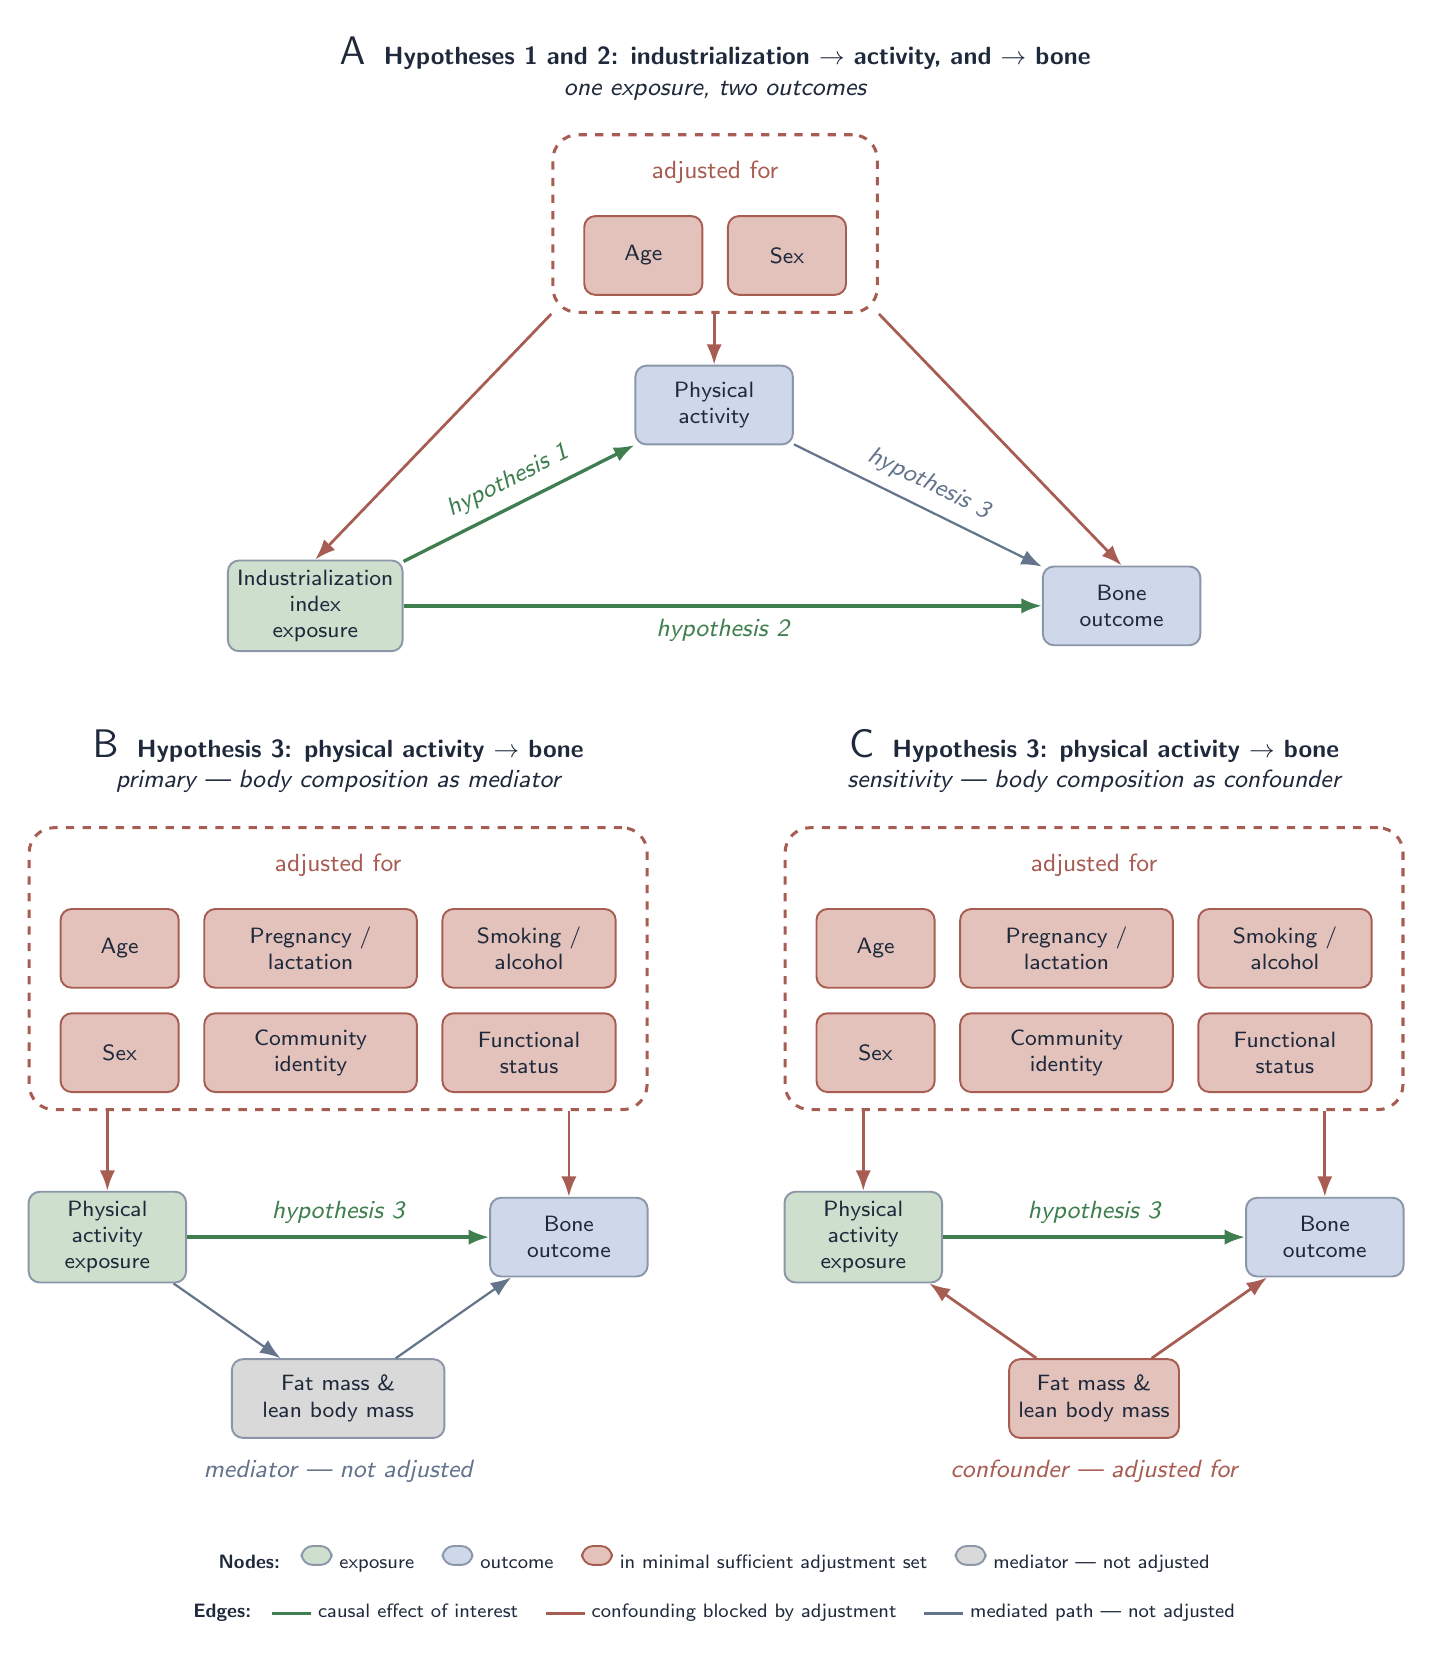
\begin{tikzpicture}

% ===== Row 1 (panel A): hypotheses 1 and 2 share the industrialization exposure =====
% Node-name suffix A matches the displayed panel letter, so the source and the figure
% cannot drift apart. Panel is centred on the two-panel row beneath it.
\begin{scope}[yshift=0cm, xshift=2.75cm]
  \node[msas] (ageA) at (3.9, 2.95) {Age};
  \node[msas, right=0.3cm of ageA] (sexA) {Sex};

  \node[anchor=south, font=\sffamily\small, text=linered] (setlabelA)
    at ($(ageA.north west)!0.5!(sexA.north east) + (0, 0.28)$)
    {adjusted for};

  % TIGHT PLATE: fits only the label and the two adjustment-set nodes, with the same
  % 11pt inner xsep panels B and C use, so the box hugs its contents identically in
  % all three panels. The panel's horizontal extent is now carried by two explicit
  % coordinates rather than by plate padding.
  \coordinate (edgeLA) at (-1.387, -1.5);
  \coordinate (edgeRA) at (10.987, -1.5);

  \begin{scope}[on background layer]
    \node[draw=linered, line width=1.1pt, dashed, rounded corners=9pt,
          fit=(setlabelA)(ageA)(sexA),
          inner xsep=11pt, inner ysep=6pt] (plateA) {};
  \end{scope}

  % Exposure at left, the two outcomes fanning right (H1 up, H2 down). All three sit at
  % distinct x so each gets its own unobstructed vertical confounding arrow, and the
  % three edge labels are pushed to different positions along their lines (pos=) so no
  % label crosses a node or another edge. The bone outcome sits well right of the
  % activity outcome to leave the hypothesis-3 label a clear run.
  % Anchored west/east on the panel-extent coordinates, which keeps the two side gaps
  % equal (the exposure node is wider than the outcome node, so any hand-set pair of
  % x centres would make the insets differ) and keeps the hypothesis-2 edge horizontal.
  \node[exposure, anchor=west] (indA)  at (edgeLA) {Industrialization\\ index\\ exposure};
  \node[outcome,  anchor=east] (boneA) at (edgeRA) {Bone\\ outcome};
  % Activity outcome centred on the gap between Age and Sex, which is also the plate's
  % centre line, so its confounding arrow drops between the two boxes.
  \node[outcome] (paA) at (4.8, 1.05) {Physical\\ activity};

  \draw[causal] (indA) -- node[anno, above, sloped, midway, text=linegreen, yshift=1pt]
        {hypothesis 1} (paA);
  \draw[causal] (indA) -- node[anno, below, midway, text=linegreen, yshift=-1pt]
        {hypothesis 2} (boneA);
  \draw[mediated] (paA) -- node[anno, above, sloped, midway, text=slate, yshift=1pt]
        {hypothesis 3} (boneA);

  % Angled out of the plate's bottom corners, terminating at each node's TOP-CENTRE.
  % Ending at the node itself (-- (indA)) aims the line at the centre but clips it
  % where it crosses the border, which for a line arriving from inboard lands the
  % arrowhead well off to one side. Naming .north puts it in the middle of the top
  % edge, which is what reads as centred. The activity outcome sits directly beneath
  % the plate, so its arrow is already vertical and centred.
  \draw[backdoor] (plateA.south west) -- (indA.north);
  \draw[backdoor] (plateA.south -| paA) -- (paA);
  \draw[backdoor] (plateA.south east) -- (boneA.north);
\end{scope}

\node[ptitle, above=3mm of plateA] {\panelid{A}\ \ Hypotheses 1 and 2: industrialization $\rightarrow$ activity, and $\rightarrow$ bone\\
  {\normalfont\itshape one exposure, two outcomes}};

% ===== Row 2 (panels B and C): the two competing structures for hypothesis 3 =====
\pabonepanel{B}{0}{-8.8}{mediator}{med}
\pabonepanel{C}{9.6}{-8.8}{msas}{conf}

\node[ptitle, above=3mm of plateB] {\panelid{B}\ \ Hypothesis 3: physical activity $\rightarrow$ bone\\
  {\normalfont\itshape primary --- body composition as mediator}};
\node[ptitle, above=3mm of plateC] {\panelid{C}\ \ Hypothesis 3: physical activity $\rightarrow$ bone\\
  {\normalfont\itshape sensitivity --- body composition as confounder}};

% ===== shared legend =====
\node[legend, text width=16cm] (legnodes) at (7.55, -13.6) {%
  \textbf{Nodes:}\ \, \lentry{exposure}{exposure} \quad
  \lentry{outcome}{outcome} \quad
  \lentry{msas}{in minimal sufficient adjustment set} \quad
  \lentry{mediator}{mediator --- not adjusted}};
\node[legend, text width=16cm, below=1.6mm of legnodes] {%
  \textbf{Edges:}\ \, \eentry{linegreen}{causal effect of interest} \quad
  \eentry{linered}{confounding blocked by adjustment} \quad
  \eentry{slate}{mediated path --- not adjusted}};

\end{tikzpicture}
\end{document}
